\documentclass{article}

\usepackage{graphicx}
\usepackage{tikz}
\usepackage{tikzsymbols}
\usetikzlibrary{calc,patterns,shapes.geometric}
\pagestyle{empty}
\usepackage[margin=0pt]{geometry}
\geometry{papersize={14in,12in}}

\def\centerarc[#1](#2)(#3:#4:#5){\draw[#1] ($(#2)+({#5*cos(#3)},{#5*sin(#3)})$) arc (#3:#4:#5);}

\begin{document}
	\begin{figure}
		\centering
		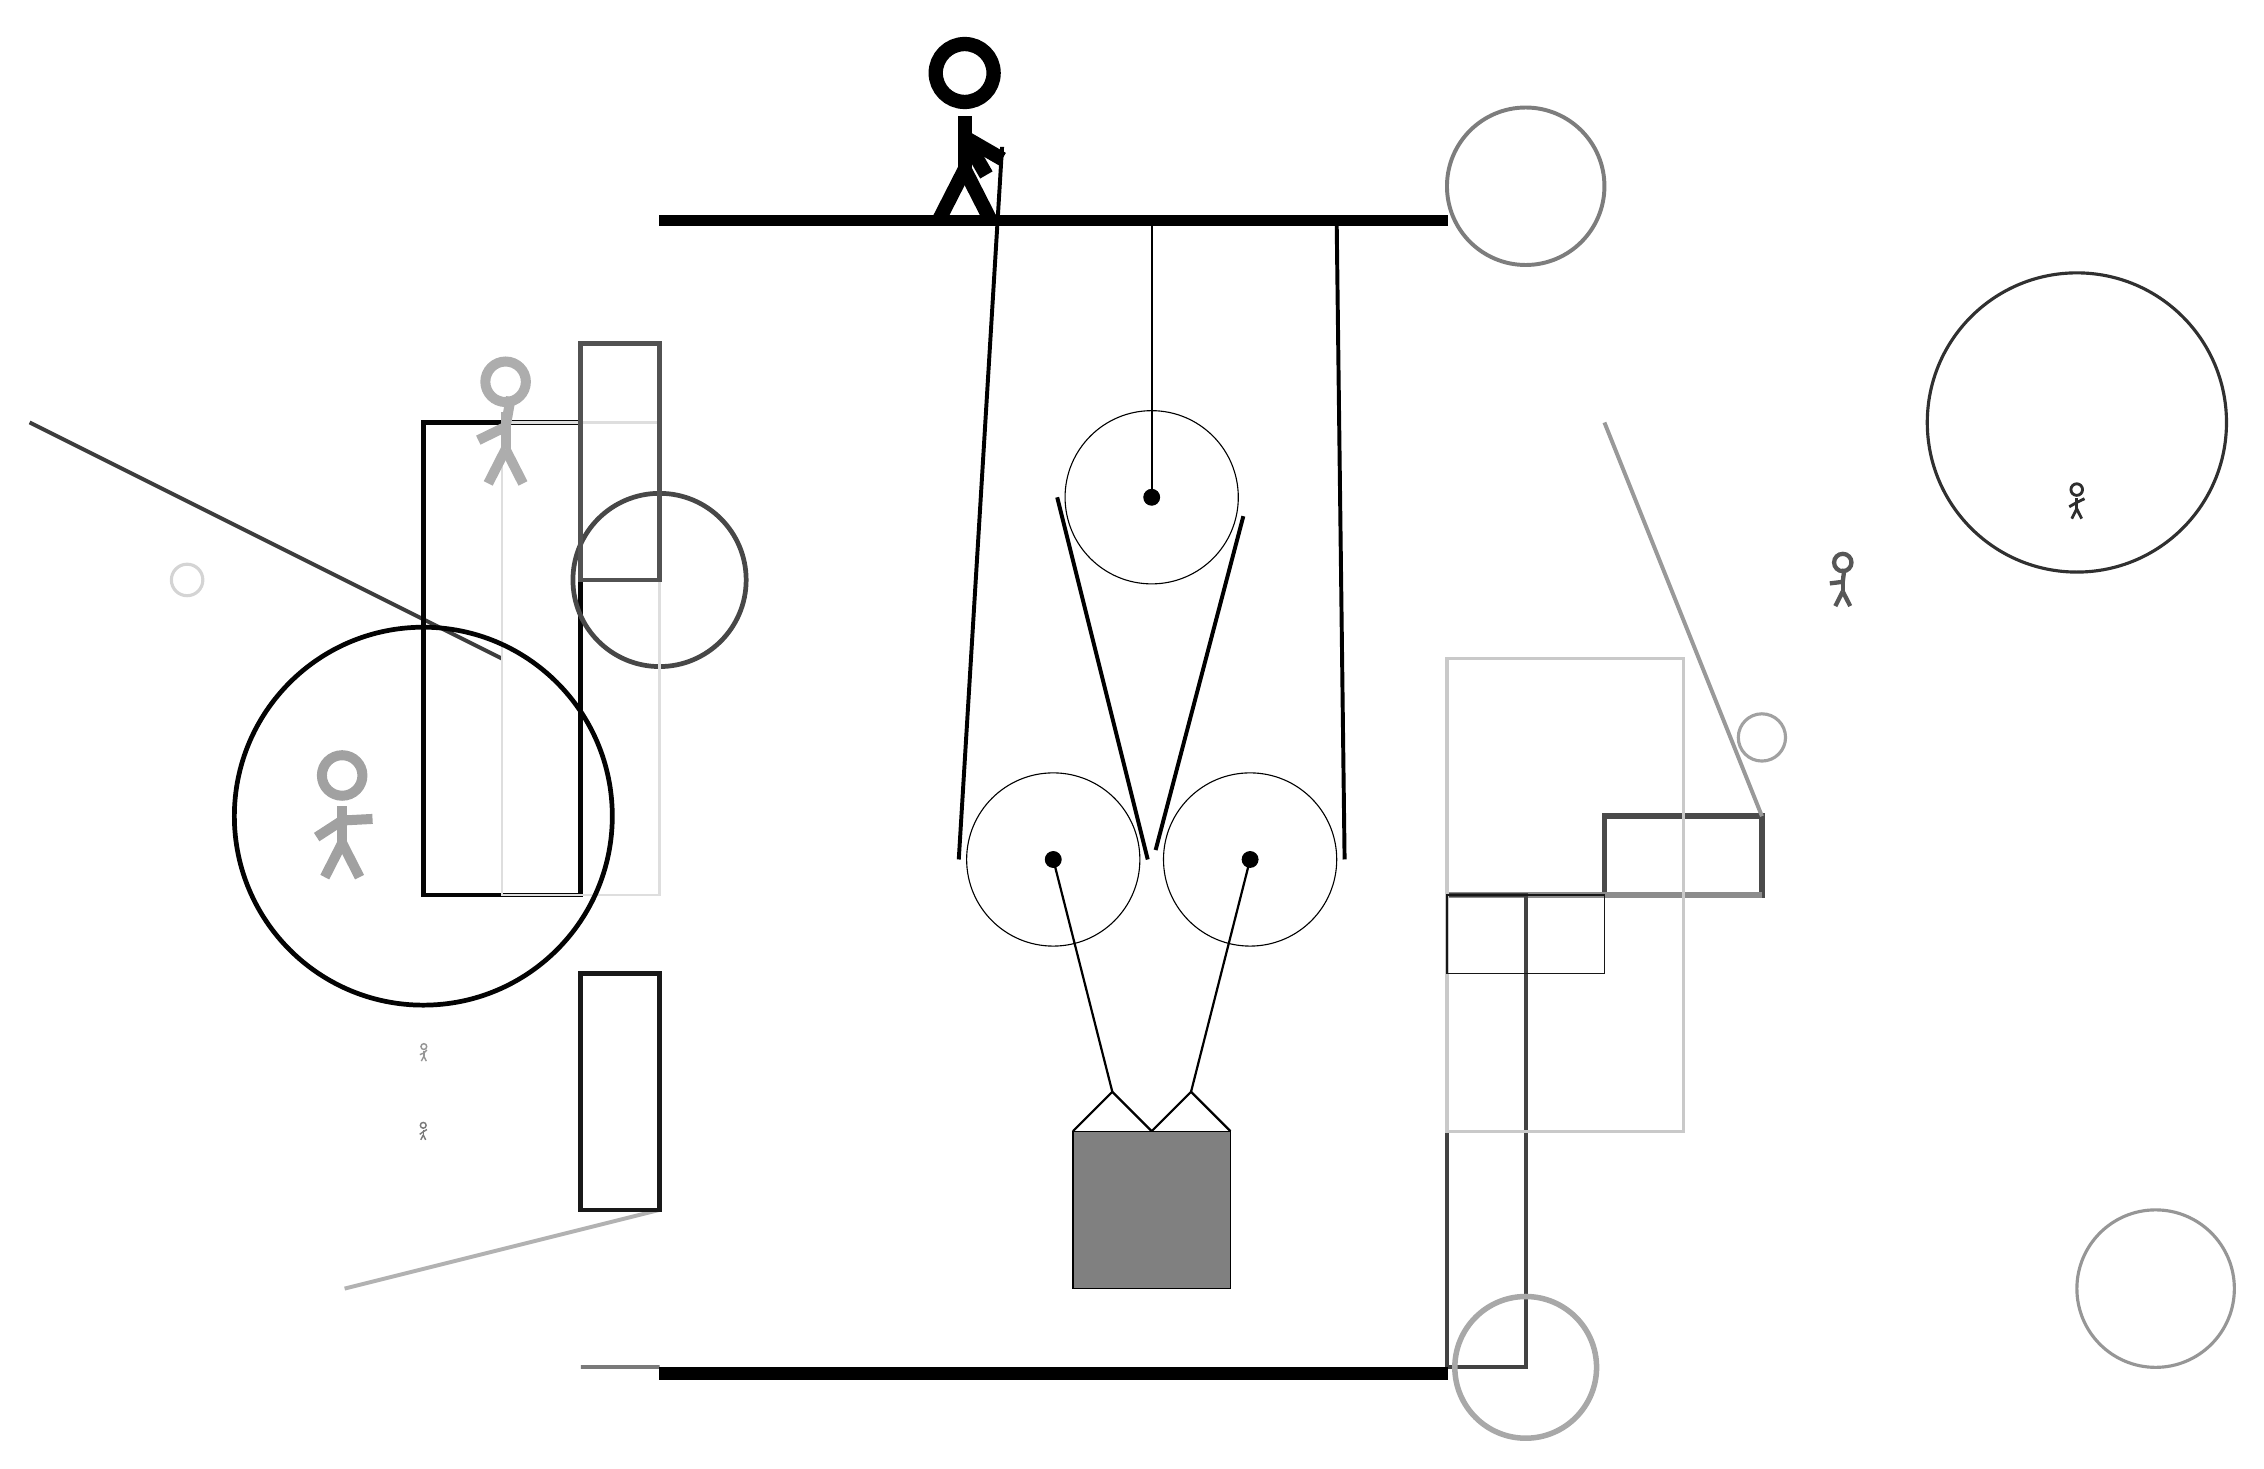
\begin{tikzpicture}
			%%%%% START %%%%%
			
			\draw[fill=black] (-4, 11.5) rectangle (6, 11.625);
			
			\node[line width=0.4mm, color=black!52] at (-7, 0) {\Strichmaxerl[1][36][31]};
			
			\draw [line width=0.5mm, color=black!51](7, 12) circle (1.0);
			\draw[line width=0.7mm, color=black!71] (8, 4) rectangle (10, 3);
			\draw[line width=0.7mm, color=black!45] (6, 3) rectangle (10, 3);
			
			\draw[line width=0.5mm, color=black!76](-6, 6) -- (-12, 9);
			
			\draw[line width=0.5mm, color=black!74] (7, 3) rectangle (6, -3);
			
			\draw[line width=0.4mm, color=black!21] (6, 0) rectangle (9, 6);
			\draw [line width=0.4mm, color=black!41](15, -2) circle (1.0);
			\draw[line width=0.6mm, color=black!98] (-5, 9) rectangle (-7, 3);
			\draw [line width=0.6mm, color=black!72](-4, 7) circle (1.1);
			
			\draw[line width=0.5mm, color=black!30](-8, -2) -- (-4, -1);
			\draw [line width=0.4mm, color=black!17](-10, 7) circle (0.2);
			\draw[line width=0.3mm, color=black!13] (-4, 3) rectangle (-6, 9);
			
			\node[line width=0.6mm, color=black!66] at (11, 7) {\Strichmaxerl[3][7][83]};
			\draw[line width=0.2mm, color=black!91] (8, 3) rectangle (6, 2);
			\node[line width=0.2mm, color=black!82] at (14, 8) {\Strichmaxerl[2][30][26]};
			\draw [line width=0.7mm, color=black!34](7, -3) circle (0.9);
			
			\draw[line width=0.5mm, color=black!52] (-5, -3) rectangle (-4, -3);
			\draw[line width=0.5mm, color=black!40](8, 9) -- (10, 4);
			\draw[line width=0.6mm, color=black!68] (-4, 10) rectangle (-5, 7);
			\draw[line width=0.6mm, color=black!90] (-5, 2) rectangle (-4, -1);
			
			\draw [line width=0.4mm, color=black!37](10, 5) circle (0.3);
			\draw [line width=0.6mm, color=black!99](-7, 4) circle (2.4);
			\node[line width=0.5mm, color=black!37] at (-8, 4) {\Strichmaxerl[7][33][3]};
			\node[line width=0.5mm, color=black!32] at (-6, 9) {\Strichmaxerl[7][26][80]};
			
			\draw [line width=0.4mm, color=black!81](14, 9) circle (1.9);
			\node[line width=0.4mm, color=black!41] at (-7, 1) {\Strichmaxerl[1][22][46]};
			
			\draw (1, 3.45) circle (1.1);
			\draw[fill=black] (1, 3.45) circle (0.1);
			
			\draw (2.25, 8.05) circle (1.1);
			\draw[fill=black] (2.25, 8.05) circle (0.1);
			\draw[thick] (2.25, 8.05) -- (2.25, 11.5);
			
			\draw (3.5, 3.45) circle (1.1);
			\draw[fill=black] (3.5, 3.45) circle (0.1);
			
			\draw[thick] (3.5, 3.45) -- (2.75, 0.5);
			\draw[thick] (1, 3.45) -- (1.75, 0.5);
			\draw[thick]  (1.25, 0) -- (1.75, 0.5) -- (2.25, 0);
			\draw[thick]  (2.25, 0) -- (2.75, 0.5) -- (3.25, 0);
			\draw[fill=black!50] (1.25, 0) rectangle (3.25, -2);
			
			\draw[line width=0.5mm] (0.35, 12.5) --  (-0.2, 3.45);
			\centerarc[line width=0.5mm](1, 3.45)(180:360:1.2000000000000002);
			\draw[line width=0.5mm] (2.2, 3.45) -- (1.05, 8.05);
			\centerarc[line width=0.5mm](2.25, 8.05)(-20:180:1.2000000000000002);
			\draw[line width=0.5mm](3.414, 7.81) -- (2.3, 3.57);
			\centerarc[line width=0.5mm](3.5, 3.45)(160:360:1.2000000000000002);
			\draw[line width=0.5mm](4.7, 3.45) -- (4.6, 11.5);
			
			\node at (-0.07, 12.7) {\Strichmaxerl[10][120][-30]};
			
			\draw[fill=black] (-4, -3) rectangle (6, -3.15);
			
			%%%%% END %%%%%
		\end{tikzpicture}
	\end{figure}	
\end{document}